\subsection{Lateral. Diaphragms/Shear walls}

\subsubsection{East and West facades shear walls}
The shear walls of the East facade are those denoted by the letters ``E'' and ``W'' in figures \ref{fg_3rd_floor_key_plan} to \ref{fg_1st_floor_key_plan}. The wind load on each floor per unit length is as follows:

\begin{center}
  \begin{tabular}{|l|c|}
    \hline
    \textbf{floor} & \textbf{wind force}\\
    & $(kN/m)$\\
    \hline
    roof & 2.34 \\
    third & 1.67 \\
    second & 1.71 \\
    \hline
  \end{tabular}
\end{center}  

\noindent The shear values obtained for each wall are as follows:

\begin{center}
  \begin{tabular}{|l|c|c|c|}
    \hline
    \textbf{floor} & \multicolumn{3}{|c|}{\textbf{shear force} $(kN)$}\\
                   & EA/WA & EB/WB & EC/WC \\
    \hline
    roof & 68.76 & -21.54 & 59.39 \\
    third & 48.93 & -15.32 & 42.26 \\
    second & 118.86 & 44.95 & 31.49 \\
    \hline
  \end{tabular}
\end{center}  

\noindent And the cumulated values are:

\begin{center}
  \begin{tabular}{|l|c|c|c|}
    \hline
    \textbf{floor} & \multicolumn{3}{|c|}{\textbf{shear force} $(kN)$}\\
                   & EA/WA & EB/WB & EC/WC \\
    \hline
    roof & 68.76 & -21.54 & 59.39 \\
    third & 117.70 & -36.86 & 101.65 \\
    second & 118.86 & 8.09 & 133.14 \\
    \hline
  \end{tabular}
\end{center}

\noindent leading to the following dimensions:

\begin{center}
  \begin{tiny}
  \begin{longtable}{|c|p{1.5cm}|c|c|c|c|c|c|c|c|c|p{3cm}|}
    \hline
    \multicolumn{9}{|c|}{}& \multicolumn{2}{p{1.1cm}|}{Bottom plate attachment (foundation)} &  Bottom plate attachment (floor to floor)\\
    \hline
    \rotatebox[origin=c]{90}{Shear wall} & \rotatebox[origin=c]{90}{Sheathing material} & \rotatebox[origin=c]{90}{Panel thickness} & \rotatebox[origin=c]{90}{Blocking} & \rotatebox[origin=c]{90}{Minimum fastener penetration} & \rotatebox[origin=c]{90}{Fastener type and size} & \rotatebox[origin=c]{90}{Panel edge fastener spacing}  & \rotatebox[origin=c]{90}{Nominal unit shear capacity $v_w$} & \rotatebox[origin=c]{90}{Hold-down anchor capacity} & \rotatebox[origin=c]{90}{Number of bolts} & \rotatebox[origin=c]{90}{Bolt spacing}  & \\
\hline
ID &  & (in) &  & (in) &  & (in) & (plf) & (kip) &  & (in) & \\
\hline
SW\_E3A & Wood structural panels – sheathing & 19/32 & YES & 1-1/2 & 10d & 4 & 1430 & 3 & - & - & wood screws 20 (d= 0.32 in) at 16 in. o/c; 46 fasteners in 2 rows.\\
\hline
SW\_E3B & Wood structural panels – sheathing & 3/8 & NO & 1-3/8 & 8d & 6 & 560 & - & - & - & 16d (d= 0.268 in) nails at 12 in. o/c; 30 fasteners in 1 row.\\
\hline
SW\_E3C & Wood structural panels – sheathing & 19/32 & YES & 1-1/2 & 10d & 4 & 1430 & 6 & - & - & SDWS log screw (d= 0.197 in) at 15 in. o/c; 32 fasteners in 2 rows.\\
\hline
SW\_E2A & Wood structural panels – sheathing & 19/32 & YES & 1-1/2 & 10d & 3 & 1860 & 7 & - & - & SDWS log screw (d= 0.197 in) at 11 in. o/c; 64 fasteners in 2 rows.\\
\hline
SW\_E2B & Wood structural panels – sheathing & 3/8 & NO & 1-3/8 & 8d & 6 & 560 & 1 & - & - & 16d (d= 0.268 in) nails at 14 in. o/c; 51 fasteners in 2 rows.\\
\hline
SW\_E2C & Wood structural panels – sheathing & 19/32 & YES & 1-1/2 & 10d & 2 & 2435 & 11 & - & - & SDWS log screw (d= 0.197 in) at 9 in. o/c; 54 fasteners in 2 rows.\\
\hline
SW\_E1A & Wood structural panels – sheathing & 19/32 & YES & 1-1/2 & 10d & 2 & 2435 & 13 & 7 & 36 & SDWS log screw (d= 0.197 in) at 7 in. o/c; 64 fasteners in 2 rows.\\
\hline
SW\_E1B & Wood structural panels – sheathing & 3/8 & NO & 1-3/8 & 8d & 6 & 560 & - & 11 & 36 & 16d (d= 0.268 in) nails at 32 in. o/c; 12 fasteners in 1 row.\\
\hline
SW\_E1C & Wood structural panels – sheathing & 19/32 & YES & 1-1/2 & 10d & 2 & 2435 & 9 & 11 & 36 & SDWS log screw (d= 0.197 in) at 10 in. o/c; 72 fasteners in 2 rows.\\
\hline
SW\_W3A & Wood structural panels – sheathing & 19/32 & YES & 1-1/2 & 10d & 4 & 1430 & 3 & - & - & wood screws 20 (d= 0.32 in) at 16 in. o/c; 46 fasteners in 2 rows.\\
\hline
SW\_W3B & Wood structural panels – sheathing & 3/8 & NO & 1-3/8 & 8d & 6 & 560 & - & - & - & 16d (d= 0.268 in) nails at 12 in. o/c; 30 fasteners in 1 row.\\
\hline
SW\_W3C & Wood structural panels – sheathing & 19/32 & YES & 1-1/2 & 10d & 4 & 1430 & 6 & - & - & SDWS log screw (d= 0.197 in) at 15 in. o/c; 32 fasteners in 2 rows.\\
\hline
SW\_W2A & Wood structural panels – sheathing & 19/32 & YES & 1-1/2 & 10d & 3 & 1860 & 7 & - & - & SDWS log screw (d= 0.197 in) at 11 in. o/c; 64 fasteners in 2 rows.\\
\hline
SW\_W2B & Wood structural panels – sheathing & 3/8 & NO & 1-3/8 & 8d & 6 & 560 & 1 & - & - & 16d (d= 0.268 in) nails at 14 in. o/c; 51 fasteners in 2 rows.\\
\hline
SW\_W2C & Wood structural panels – sheathing & 19/32 & YES & 1-1/2 & 10d & 2 & 2435 & 11 & - & - & SDWS log screw (d= 0.197 in) at 9 in. o/c; 54 fasteners in 2 rows.\\
\hline
SW\_W1A & Wood structural panels – sheathing & 19/32 & YES & 1-1/2 & 10d & 2 & 2435 & 13 & 9 & 30 & SDWS log screw (d= 0.197 in) at 7 in. o/c; 64 fasteners in 2 rows.\\
\hline
SW\_W1B & Wood structural panels – sheathing & 3/8 & NO & 1-3/8 & 8d & 6 & 560 & - & 11 & 36 & 16d (d= 0.268 in) nails at 32 in. o/c; 12 fasteners in 1 row.\\
\hline
SW\_W1C & Wood structural panels – sheathing & 19/32 & YES & 1-1/2 & 10d & 2 & 2435 & 9 & 11 & 36 & SDWS log screw (d= 0.197 in) at 10 in. o/c; 72 fasteners in 2 rows.\\
    \hline
  \end{longtable}
  \end{tiny}
  \end{center}

\subsubsection{Courtyard facades shear walls}
The shear walls of the courtyard East and West facades are those denoted by the letters ``EC'' or ``WC'' in figures \ref{fg_3rd_floor_key_plan} to \ref{fg_1st_floor_key_plan}. The wind load on each floor per unit length is as follows:

\begin{center}
  \begin{tabular}{|l|c|}
    \hline
    \textbf{floor} & \textbf{wind force}\\
    & $(kN/m)$\\
    \hline
    roof & 2.50 \\
    third & 1.98 \\
    second & 2.03 \\
    \hline
  \end{tabular}
\end{center}  

\noindent The shear values obtained for each wall are as follows:

\begin{center}
  \begin{tabular}{|l|c|c|c|}
    \hline
    \textbf{floor} & \multicolumn{3}{|c|}{\textbf{shear force} $(kN)$}\\
                   & ECA/WCA & ECB/WCB & ECC/WCC \\
    \hline
    roof & 30.35 & -4.77 & 59.26 \\
    third & 24.06 & -3.78 & 46.97 \\
    second & 24.61 & -3.87 & 48.04 \\
    \hline
  \end{tabular}
\end{center}  

\noindent And the cumulated values are:

\begin{center}
  \begin{tabular}{|l|c|c|c|}
    \hline
    \textbf{floor} & \multicolumn{3}{|c|}{\textbf{shear force} $(kN)$}\\
                   & ECA/WCA & ECB/WCB & ECC/WCC \\
    \hline
roof & 30.35 & -4.77 & 59.26 \\
third & 54.41 & -8.56 & 106.22 \\
second & 79.02 & -12.43 & 154.27 \\
    \hline
  \end{tabular}
\end{center}

\noindent leading to the following dimensions:

\begin{center}
  \begin{tiny}
  \begin{longtable}{|c|p{1.5cm}|c|c|c|c|c|c|c|c|c|p{3cm}|}
    \hline
    \multicolumn{9}{|c|}{}& \multicolumn{2}{p{1.1cm}|}{Bottom plate attachment (foundation)} &  Bottom plate attachment (floor to floor)\\
    \hline
    \rotatebox[origin=c]{90}{Shear wall} & \rotatebox[origin=c]{90}{Sheathing material} & \rotatebox[origin=c]{90}{Panel thickness} & \rotatebox[origin=c]{90}{Blocking} & \rotatebox[origin=c]{90}{Minimum fastener penetration} & \rotatebox[origin=c]{90}{Fastener type and size} & \rotatebox[origin=c]{90}{Panel edge fastener spacing}  & \rotatebox[origin=c]{90}{Nominal unit shear capacity $v_w$} & \rotatebox[origin=c]{90}{Hold-down anchor capacity} & \rotatebox[origin=c]{90}{Number of bolts} & \rotatebox[origin=c]{90}{Bolt spacing}  & \\
\hline
ID &  & (in) &  & (in) &  & (in) & (plf) & (kip) &  & (in) & \\
\hline
SW\_EC3A & Wood structural panels – sheathing & 19/32 & YES & 1-1/2 & 10d & 6 & 950 & 0 & - & - & 16d (d= 0.268 in) nails at 18 in. o/c; 42 fasteners in 2 rows.\\
\hline
SW\_EC3B & Wood structural panels – sheathing & 3/8 & NO & 1-3/8 & 8d & 6 & 560 & - & - & - & 16d (d= 0.268 in) nails at 60 in. o/c; 7 fasteners in 1 row.\\
\hline
SW\_EC3C & Wood structural panels – sheathing & 19/32 & YES & 1-1/2 & 10d & 6 & 950 & 3 & - & - & wood screws 20 (d= 0.32 in) at 19 in. o/c; 40 fasteners in 2 rows.\\
\hline
SW\_EC2A & Wood structural panels – sheathing & 19/32 & YES & 1-1/2 & 10d & 3 & 1860 & 2 & - & - & wood screws 20 (d= 0.32 in) at 21 in. o/c; 36 fasteners in 2 rows.\\
\hline
SW\_EC2B & Wood structural panels – sheathing & 3/8 & NO & 1-3/8 & 8d & 6 & 560 & - & - & - & 16d (d= 0.268 in) nails at 32 in. o/c; 12 fasteners in 1 row.\\
\hline
SW\_EC2C & Wood structural panels – sheathing & 19/32 & YES & 1-1/2 & 10d & 3 & 1860 & 6 & - & - & SDWS log screw (d= 0.197 in) at 12 in. o/c; 58 fasteners in 2 rows.\\
\hline
SW\_EC1A & Wood structural panels – sheathing & 19/32 & YES & 1-1/2 & 10d & 2 & 2435 & 11 & 6 & 36 & SDWS log screw (d= 0.197 in) at 9 in. o/c; 42 fasteners in 2 rows.\\
\hline
SW\_EC1B & Wood structural panels – sheathing & 3/8 & NO & 1-3/8 & 8d & 6 & 560 & - & 11 & 36 & 16d (d= 0.268 in) nails at 22 in. o/c; 17 fasteners in 1 row.\\
\hline
SW\_EC1C & Wood structural panels – sheathing & 19/32 & YES & 1-1/2 & 10d & 2 & 2435 & 11 & 11 & 36 & SDWS log screw (d= 0.197 in) at 9 in. o/c; 82 fasteners in 2 rows.\\
\hline
SW\_WC3A & Wood structural panels – sheathing & 19/32 & YES & 1-1/2 & 10d & 6 & 950 & 0 & - & - & 16d (d= 0.268 in) nails at 18 in. o/c; 42 fasteners in 2 rows.\\
\hline
SW\_WC3B & Wood structural panels – sheathing & 3/8 & NO & 1-3/8 & 8d & 0 & 560 & - & - & - & 16d (d= 0.268 in) nails at 60 in. o/c; 7 fasteners in 1 row.\\
\hline
SW\_WC3C & Wood structural panels – sheathing & 19/32 & YES & 1-1/2 & 10d & 6 & 950 & 3 & - & - & wood screws 20 (d= 0.32 in) at 19 in. o/c; 40 fasteners in 2 rows.\\
\hline
SW\_WC2A & Wood structural panels – sheathing & 19/32 & YES & 1-1/2 & 10d & 3 & 1860 & 2 & - & - & wood screws 20 (d= 0.32 in) at 21 in. o/c; 36 fasteners in 2 rows.\\
\hline
SW\_WC2B & Wood structural panels – sheathing & 3/8 & NO & 1-3/8 & 8d & 6 & 560 & - & - & - & 16d (d= 0.268 in) nails at 32 in. o/c; 12 fasteners in 1 row.\\
\hline
SW\_WC2C & Wood structural panels – sheathing & 19/32 & YES & 1-1/2 & 10d & 3 & 1860 & 6 & - & - & SDWS log screw (d= 0.197 in) at 12 in. o/c; 58 fasteners in 2 rows.\\
\hline
SW\_WC1A & Wood structural panels – sheathing & 19/32 & YES & 1-1/2 & 10d & 2 & 2435 & 11 & 6 & 36 & SDWS log screw (d= 0.197 in) at 9 in. o/c; 42 fasteners in 2 rows.\\
\hline
SW\_WC1B & Wood structural panels – sheathing & 3/8 & NO & 1-3/8 & 8d & 6 & 560 & - & 11 & 36 & 16d (d= 0.268 in) nails at 22 in. o/c; 17 fasteners in 1 row.\\
\hline
SW\_WC1C & Wood structural panels – sheathing & 19/32 & YES & 1-1/2 & 10d & 2 & 2435 & 11 & 11 & 36 & SDWS log screw (d= 0.197 in) at 9 in. o/c; 82 fasteners in 2 rows.\\
    \hline
  \end{longtable}
  \end{tiny}
  \end{center}

\subsubsection{South facades shear walls}
The shear walls of the South facade are those denoted by the letter ``S'' in figures \ref{fg_3rd_floor_key_plan} to \ref{fg_1st_floor_key_plan}. The wind load on each floor per unit length is as follows:

\begin{center}
  \begin{tabular}{|l|c|}
    \hline
    \textbf{floor} & \textbf{wind force}\\
    & $(kN/m)$\\
    \hline
    roof & 2.50 \\
    third & 1.98 \\
    second & 2.03 \\
    \hline
  \end{tabular}
\end{center}  

\noindent The shear values obtained for each wall are as follows:

\begin{center}
  \begin{tabular}{|l|c|}
    \hline
    \textbf{floor} & \textbf{shear force} $(kN)$\\
                   & SA/SB \\
    \hline
    roof & 54.95 \\
    third & 43.56 \\
    second & 44.55 \\
    \hline
  \end{tabular}
\end{center}  

\noindent And the cumulated values are:

\begin{center}
  \begin{tabular}{|l|c|}
    \hline
    \textbf{floor} & \textbf{shear force} $(kN)$\\
                   & SA/SB \\
    \hline
    roof & 54.95 \\
    third & 98.51 \\
    second & 143.06 \\
    \hline
  \end{tabular}
\end{center}  

\noindent leading to the following dimensions:
\begin{center}
  \begin{tiny}
  \begin{longtable}{|c|p{1.5cm}|c|c|c|c|c|c|c|c|c|p{3cm}|}
    \hline
    \multicolumn{9}{|c|}{}& \multicolumn{2}{p{1.1cm}|}{Bottom plate attachment (foundation)} &  Bottom plate attachment (floor to floor)\\
    \hline
    \rotatebox[origin=c]{90}{Shear wall} & \rotatebox[origin=c]{90}{Sheathing material} & \rotatebox[origin=c]{90}{Panel thickness} & \rotatebox[origin=c]{90}{Blocking} & \rotatebox[origin=c]{90}{Minimum fastener penetration} & \rotatebox[origin=c]{90}{Fastener type and size} & \rotatebox[origin=c]{90}{Panel edge fastener spacing}  & \rotatebox[origin=c]{90}{Nominal unit shear capacity $v_w$} & \rotatebox[origin=c]{90}{Hold-down anchor capacity} & \rotatebox[origin=c]{90}{Number of bolts} & \rotatebox[origin=c]{90}{Bolt spacing}  & \\
\hline
ID &  & (in) &  & (in) &  & (in) & (plf) & (kip) &  & (in) & \\
\hline
SW\_S3A & Wood structural panels – sheathing & 19/32 & YES & 1-1/2 & 10d & 6 & 950 & 2 & - & - & wood screws 20 (d= 0.32 in) at 21 in. o/c; 36 fasteners in 2 rows.\\
\hline
SW\_S3B & Wood structural panels – sheathing & 19/32 & YES & 1-1/2 & 10d & 6 & 950 & 2 & - & - & wood screws 20 (d= 0.32 in) at 21 in. o/c; 36 fasteners in 2 rows.\\
\hline
SW\_S2A & Wood structural panels – sheathing & 19/32 & YES & 1-1/2 & 10d & 3 & 1860 & 6 & - & - & SDWS log screw (d= 0.197 in) at 13 in. o/c; 54 fasteners in 2 rows.\\
\hline
SW\_S2B & Wood structural panels – sheathing & 19/32 & YES & 1-1/2 & 10d & 3 & 1860 & 6 & - & - & SDWS log screw (d= 0.197 in) at 13 in. o/c; 54 fasteners in 2 rows.\\
\hline
SW\_S1A & Wood structural panels – sheathing & 19/32 & YES & 1-1/2 & 10d & 2 & 2435 & 11 & 10 & 36 & SDWS log screw (d= 0.197 in) at 8 in. o/c; 76 fasteners in 2 rows.\\
\hline
SW\_S1B & Wood structural panels – sheathing & 19/32 & YES & 1-1/2 & 10d & 2 & 2435 & 11 & 10 & 36 & SDWS log screw (d= 0.197 in) at 8 in. o/c; 76 fasteners in 2 rows.\\
\hline
\hline
  \end{longtable}
  \end{tiny}
  \end{center}

\subsubsection{North facade shear walls}
The shear walls of the North facade are those denoted by the letter ``N'' in figures \ref{fg_3rd_floor_key_plan} to \ref{fg_1st_floor_key_plan}. The wind load on each floor per unit length is as follows:


\begin{center}
  \begin{tabular}{|l|c|}
    \hline
    \textbf{floor} & \textbf{wind force}\\
    & $(kN/m)$\\
    \hline
    roof & 2.34 \\
    third & 1.67 \\
    second & 1.71 \\
    \hline
  \end{tabular}
\end{center}

\noindent The shear values obtained for each wall are as follows:

\begin{center}
  \begin{tabular}{|l|c|c|c|c|}
    \hline
    \textbf{floor} & \multicolumn{4}{|c|}{\textbf{shear force} $(kN)$}\\
                   & NA & NB & NC & ND \\
    \hline
    roof & 44.84 & 11.72 & 25.01 & 45.63 \\
    third & 31.91 & 8.34 & 17.79 & 32.47 \\
    second & 32.64 & 8.53 & 18.20 & 33.22 \\
    \hline
  \end{tabular}
\end{center}  

\noindent And the cumulated values are:

\begin{center}
  \begin{tabular}{|l|c|c|c|c|}
    \hline
    \textbf{floor} & \multicolumn{4}{|c|}{\textbf{shear force} $(kN)$}\\
                   & NA & NB & NC & ND \\
    \hline
    roof & 44.84 & 11.72 & 25.01 & 45.63 \\
    third & 76.75 & 20.06 & 42.80 & 78.11 \\
    second & 109.39 & 28.59 & 61.01 & 111.33 \\
    \hline
  \end{tabular}
\end{center}  

\noindent leading to the following dimensions:
\begin{center}
  \begin{tiny}
  \begin{longtable}{|c|p{1.5cm}|c|c|c|c|c|c|c|c|c|p{3cm}|}
    \hline
    \multicolumn{9}{|c|}{}& \multicolumn{2}{p{1.1cm}|}{Bottom plate attachment (foundation)} &  Bottom plate attachment (floor to floor)\\
    \hline
    \rotatebox[origin=c]{90}{Shear wall} & \rotatebox[origin=c]{90}{Sheathing material} & \rotatebox[origin=c]{90}{Panel thickness} & \rotatebox[origin=c]{90}{Blocking} & \rotatebox[origin=c]{90}{Minimum fastener penetration} & \rotatebox[origin=c]{90}{Fastener type and size} & \rotatebox[origin=c]{90}{Panel edge fastener spacing}  & \rotatebox[origin=c]{90}{Nominal unit shear capacity $v_w$} & \rotatebox[origin=c]{90}{Hold-down anchor capacity} & \rotatebox[origin=c]{90}{Number of bolts} & \rotatebox[origin=c]{90}{Bolt spacing}  & \\
\hline
ID &  & (in) &  & (in) &  & (in) & (plf) & (kip) &  & (in) & \\
SW\_N3A & Wood structural panels – sheathing & 3/8 & YES & 1-3/8 & 8d & 4 & 840 & 2 & - & - & wood screws 20 (d= 0.32 in) at 25 in. o/c; 30 fasteners in 2 rows.\\
\hline
SW\_N3B & Wood structural panels – sheathing & 3/8 & NO & 1-3/8 & 8d & 6 & 560 & - & - & - & 16d (d= 0.268 in) nails at 24 in. o/c; 16 fasteners in 1 row.\\
\hline
SW\_N3C & Wood structural panels – sheathing & 3/8 & NO & 1-3/8 & 8d & 6 & 560 & - & - & - & 16d (d= 0.268 in) nails at 21 in. o/c; 35 fasteners in 2 rows.\\
\hline
SW\_N3D & Wood structural panels – sheathing & 3/8 & YES & 1-3/8 & 8d & 4 & 840 & 2 & - & - & wood screws 20 (d= 0.32 in) at 25 in. o/c; 30 fasteners in 2 rows.\\
\hline
SW\_N2A & Wood structural panels – sheathing & 19/32 & YES & 1-1/2 & 10d & 4 & 1430 & 4 & - & - & wood screws 20 (d= 0.32 in) at 14 in. o/c; 52 fasteners in 2 rows.\\
\hline
SW\_N2B & Wood structural panels – sheathing & 19/32 & YES & 1-1/2 & 10d & 6 & 950 & - & - & - & 16d (d= 0.268 in) nails at 13 in. o/c; 28 fasteners in 1 row.\\
\hline
SW\_N2C & Wood structural panels – sheathing & 19/32 & YES & 1-1/2 & 10d & 6 & 950 & 1 & - & - & 16d (d= 0.268 in) nails at 12 in. o/c; 59 fasteners in 2 rows.\\
\hline
SW\_N2D & Wood structural panels – sheathing & 19/32 & YES & 1-1/2 & 10d & 4 & 1430 & 4 & - & - & wood screws 20 (d= 0.32 in) at 14 in. o/c; 52 fasteners in 2 rows.\\
\hline
SW\_N1A & Wood structural panels – sheathing & 19/32 & YES & 1-1/2 & 10d & 3 & 1860 & 7 & 10 & 36 & SDWS log screw (d= 0.197 in) at 12 in. o/c; 58 fasteners in 2 rows.\\
\hline
SW\_N1B & Wood structural panels – sheathing & 19/32 & YES & 1-1/2 & 10d & 6 & 950 & - & 11 & 36 & 16d (d= 0.268 in) nails at 19 in. o/c; 39 fasteners in 2 rows.\\
\hline
SW\_N1C & Wood structural panels – sheathing & 19/32 & YES & 1-1/2 & 10d & 6 & 950 & 3 & 11 & 36 & wood screws 20 (d= 0.32 in) at 19 in. o/c; 40 fasteners in 2 rows.\\
\hline
SW\_N1D & Wood structural panels – sheathing & 19/32 & YES & 1-1/2 & 10d & 3 & 1860 & 7 & 10 & 36 & SDWS log screw (d= 0.197 in) at 12 in. o/c; 60 fasteners in 2 rows.\\
\hline
  \end{longtable}
  \end{tiny}
  \end{center}

\begin{figure}
  \begin{center}
  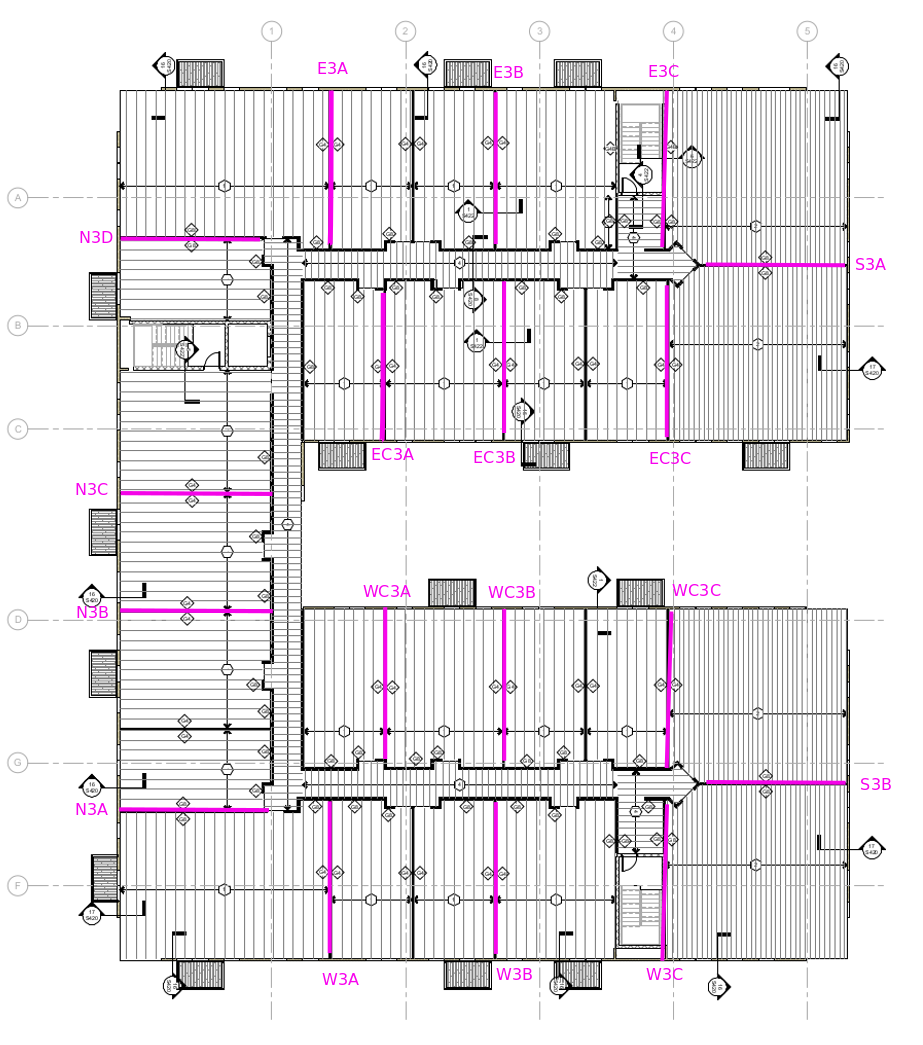
\includegraphics[width=120mm]{figures/3rd_floor_key_plan}
  \end{center}
  \caption{Shear walls on the third floor.}\label{fg_3rd_floor_key_plan}
\end{figure}

\begin{figure}
  \begin{center}
  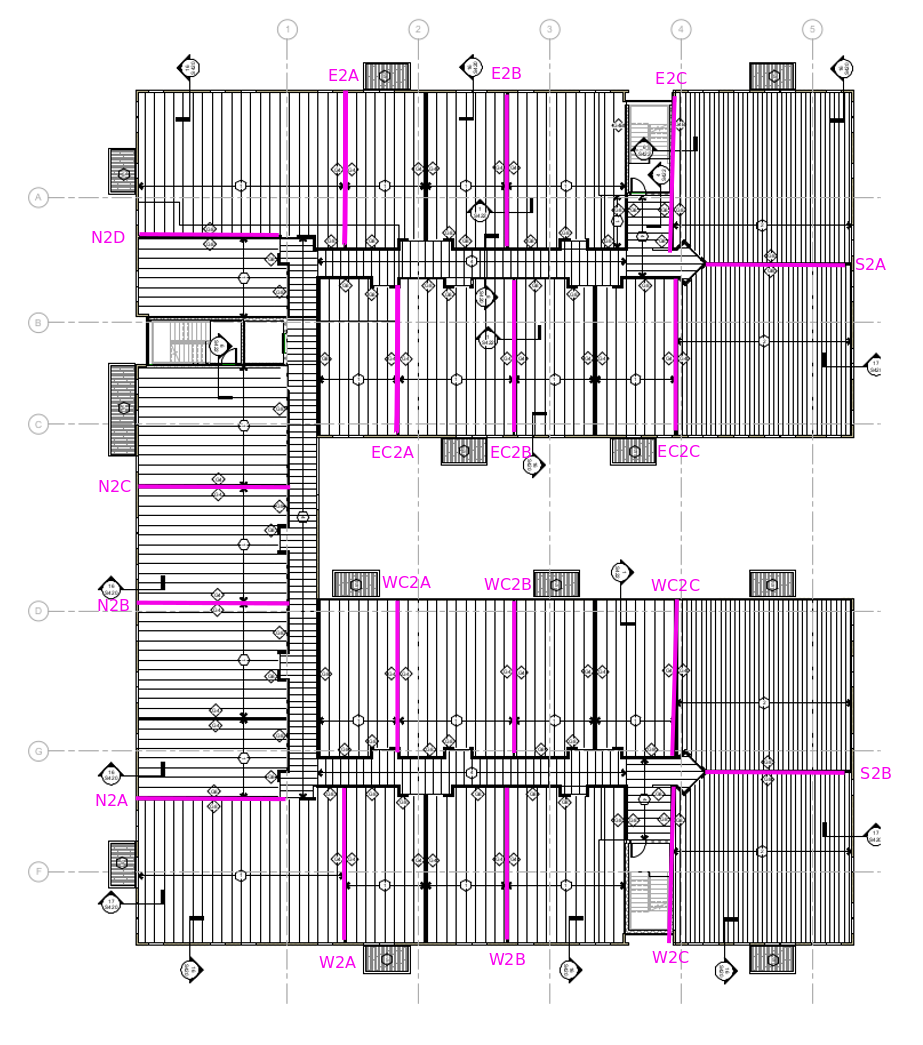
\includegraphics[width=120mm]{figures/2nd_floor_key_plan}
  \end{center}
  \caption{Shear walls on the second floor.}\label{fg_2nd_floor_key_plan}
\end{figure}


\begin{figure}
  \begin{center}
  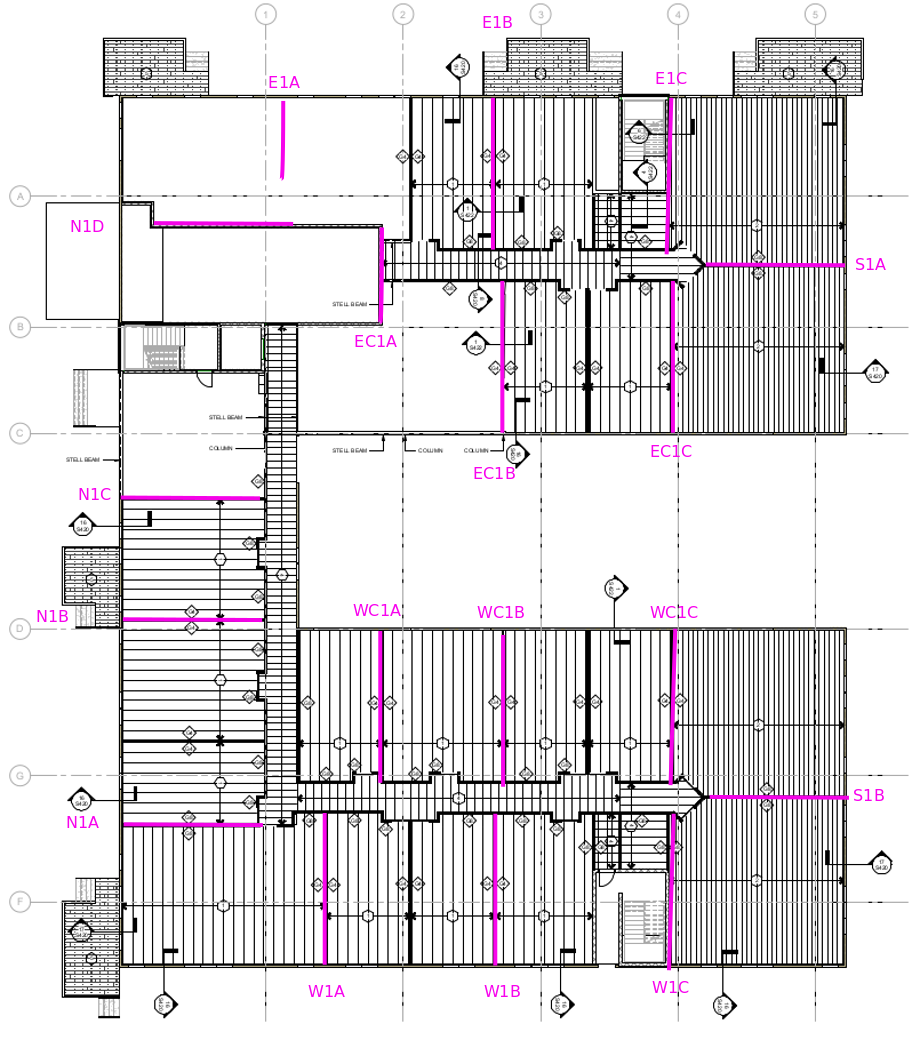
\includegraphics[width=120mm]{figures/1st_floor_key_plan}
  \end{center}
  \caption{Shear walls on the first floor.}\label{fg_1st_floor_key_plan}
\end{figure}
